With the goal to recognize facial expressions in images, we need to detect faces within them then extract their features so we expect the input image to have \textbf{good quality, sharpness and clearness} as much as possible.\newline
Fortunately nowadays cameras have higher quality so in this case there should be no problem, however in case of low quality input images we need to apply some enhancement techniques before we proceed to subsequent stages.

\paragraph{Most common problems}
\subparagraph{Salt and Pepper Noise}
It is a form of noise sometimes seen on images, it is also known as impulse noise, this noise can be caused by sharp and sudden disturbances in the image signal, it presents itself as sparsely occurring white and black pixels.\newline
An effective noise reduction method for this type of noise is a \textbf{Median Filter}.\newline
The main idea of the Median Filter is replacing each pixel with the median of neighboring pixels, the pattern of neighbors is called the "window", which slides, entry by entry, over the entire photo.(see Figure~\ref{fig:median})


\begin{figure}%[H]
	\centering
	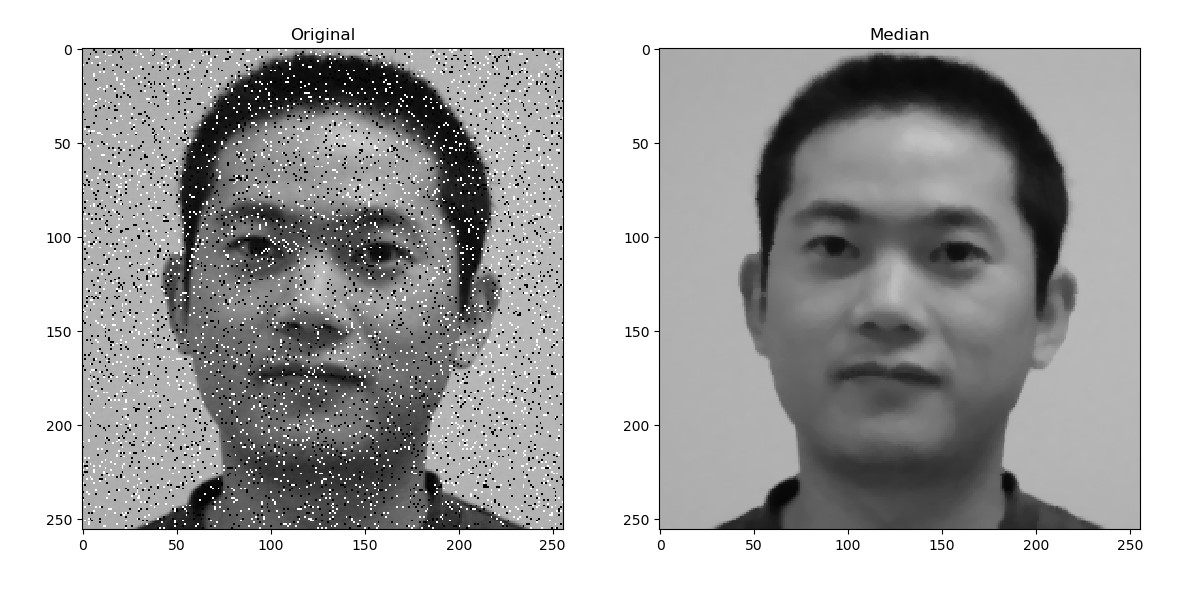
\includegraphics[width=.5\linewidth]{images/salt_pepper.jpg}
	\caption{Apply Median Filter on salt and paper noise}
	\label{fig:median}
\end{figure}

\subparagraph{Gaussian Noise}
It is a type of noise that has a probability density function (PDF) that follows normal distribution, an effective noise reduction method for this type of noise is a \textbf{Non-local Means Denoising Algorithm}.\newline
We need a set of similar images to average out the noise, consider a small window (say 5x5 window) in the image. Chance is large that the same patch may be somewhere else in the image. Sometimes in a small neighborhood around it. What about using these similar patches together and find their average.\newline
The blue patches in the image looks the similar, green patches looks similar, so we take a pixel, take small window around it, search for similar windows in the image, average all the windows and replace the pixel with the result we got (see Figure~\ref{fig:Gnoise}).\newline 

\begin{figure}[H]
	\centering
	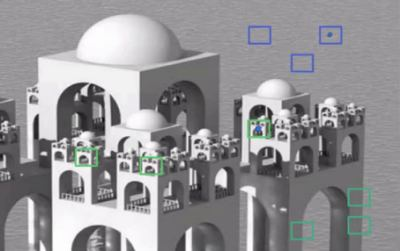
\includegraphics[width=.5\linewidth]{images/nlmd.jpg}
\end{figure}

\begin{figure}[H]
	\centering
	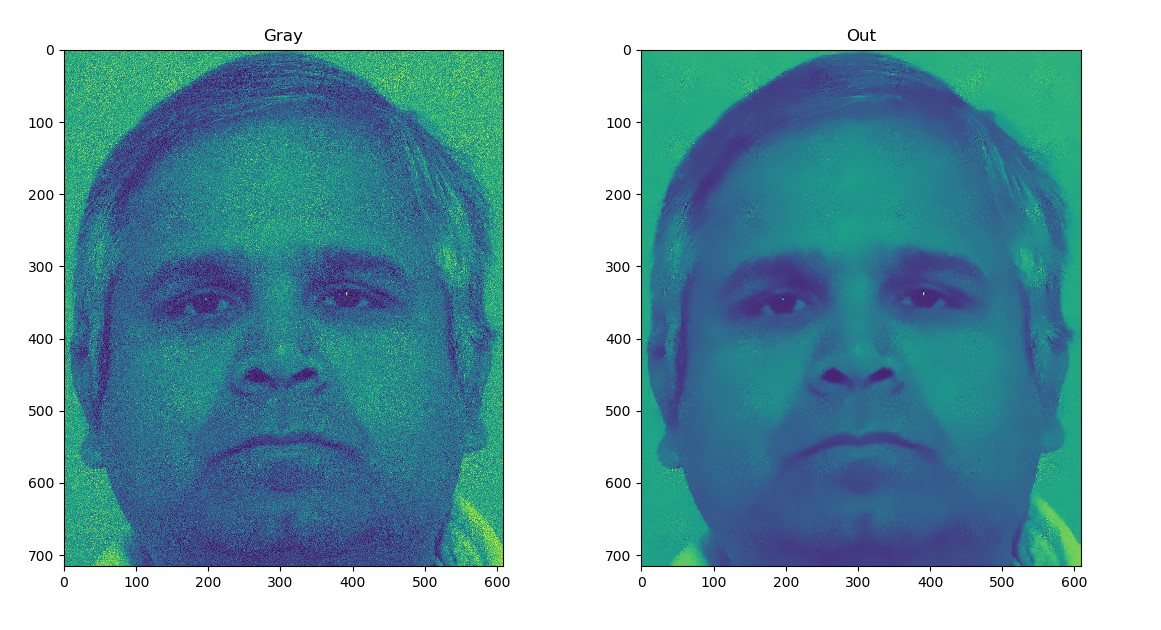
\includegraphics[width=.5\linewidth]{images/gaussian.jpg}
	\caption{Gaussian noise and patch concept example}
	\label{fig:Gnoise}
\end{figure}

\subparagraph{Smoothed Images:}
Some images can be blurred which hides small details within them, an effective noise reduction method for this type of noise is a \textbf{Sharpening Spatial Filter}.\newline
Sharpening spatial filters seek to \textbf{highlight small details by removing blur from images and Highlighting edges} within them.(see Figure~\ref{figure:laplacian})\newline
Sharpening filters are based on spatial differentiation.\newline
The Laplacian is defined as follows:
\[\nabla^{2} f = \frac{\partial^{2}f}{\partial^{2}x} + \frac{\partial^{2}f}{\partial^{2}y}\]

Where the partial 2nd order derivative in the x direction is defined as follows:
\[\frac{\partial^{2}f}{\partial^{2}x} = f(x+1, y) + f(x-1, y) - 2f(x, y)\]

And in the y direction as follows:
\[\frac{\partial^{2}f}{\partial^{2}x} = f(x, y+1) + f(x, y-1) - 2f(x, y)\]

So, the Laplacian can be given as follows:
\[\nabla^{2} f = f(x+1, y) + f(x-1, y) + f(x, y+1) + f(x, y-1) - 4f(x, y)\]

We can build a filter based on this:
\[
\begin{bmatrix}
0 & 1 & 0 \\
1 & -4 & 1 \\
0 & 1 & 0
\end{bmatrix} \]
Which is the laplacian filter, to get the sharpened image we subtract the output of laplacian filter from the original image.
\[g(x, y) = f(x, y) - \nabla^{2} f\]

By combining the two steps together we reach the sharpening filter
\[
\begin{bmatrix}
0 & -1 & 0 \\
-1 & 5 & -1 \\
0 & -1 & 0
\end{bmatrix} \]

Sharpening filters has multiple similar variations we use the one below as it gives better results.
\[
\begin{bmatrix}
-1 & -1 & -1 \\
-1 & 9 & -1 \\
-1 & -1 & -1
\end{bmatrix} \]

\begin{figure}[H]
	\centering
	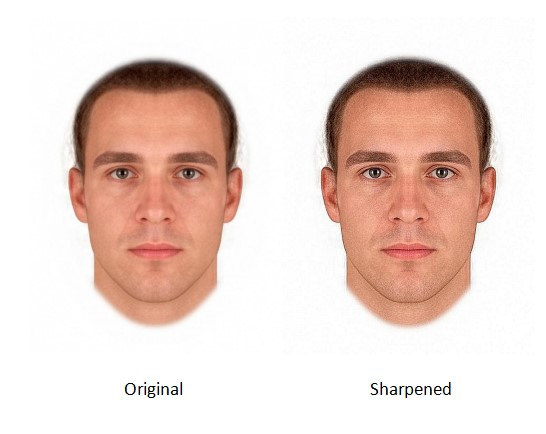
\includegraphics[width=0.5\linewidth]{images/Sharpened.jpg}
	\caption{Laplacian Filter Example}
	\label{figure:laplacian}
\end{figure}

\subparagraph{Motion Blurred Images:}
It is the apparent streaking of moving objects in an image or a sequence of frames, such as a film or animation, It results when the image being recorded changes during the recording of a single exposure, due to rapid movement or long exposure.\newline
An effective noise reduction method for this type of noise is a trained model called \textbf{Keras Deblur GAN}.\newline
\begin{figure}[H]
	\centering
	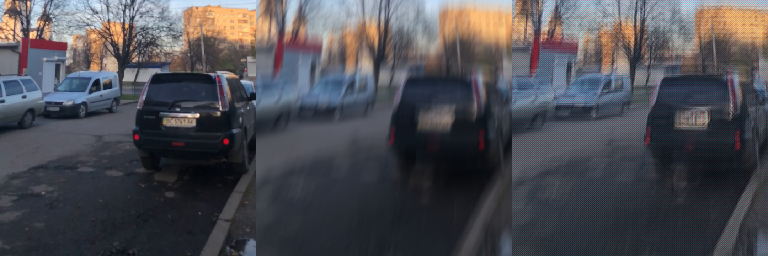
\includegraphics[width=0.7\linewidth]{images/motion_blur.png}
	\caption{Motion Blur Example}
\end{figure}

\subparagraph{Face alignment:}
We prefer to deal with frontal faces to easily detect them, but sometimes faces aren’t necessarily aligned in that way, so we may use a trained model called FaceAligner in OpenCV library which rotates the image such that the eyes lie on a horizontal line (i.e., the eyes lie along the same y-coordinates).\newline
\begin{figure}[H]
	\centering
	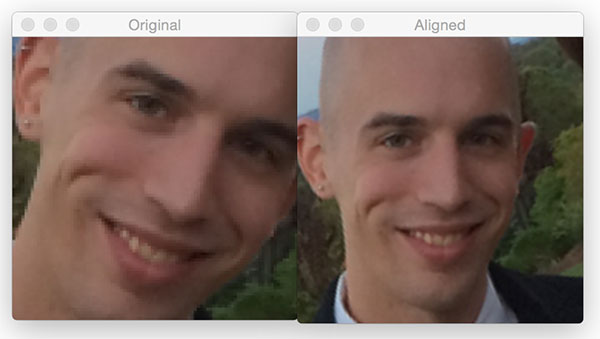
\includegraphics[width=0.7\linewidth]{images/Aligning.jpg}
	\caption{Aligning Example}
\end{figure}
